\documentclass[a4paper,11pt]{article}
\usepackage[italian]{babel}
\usepackage[utf8]{inputenc}
\usepackage{csquotes}
\usepackage[margin = 1.4in]{geometry}
\usepackage{amsmath}
\usepackage{centernot}
\usepackage{amsfonts}
\usepackage{placeins}
\usepackage{tcolorbox}
\usepackage{float}
\usepackage[font=scriptsize]{caption}
\usepackage[table,xcdraw]{xcolor}
\usepackage[framemethod=tikz]{mdframed}
\usepackage[
backend=biber,
style=alphabetic,
]{biblatex}
\addbibresource{citations.bib}
\newmdenv[innerlinewidth=0.5pt,roundcorner=4pt,linecolor=lightgray,innerleftmargin=6pt,
innerrightmargin=6pt,innertopmargin=6pt,innerbottommargin=6pt]{myblock}
\begin{document}
\title{\textbf{Circuito tosatore a due livelli}

1° turno tavolo 5}
\author{Stefano Doria 0001093903 \and Giuseppe Luciano 0001077643}

\date{Marzo 2025}

\maketitle

\section{Abstract}

L'esperimento aveva come fine quello di realizzare un circuito di doppio clipping, realizzato sia con diodi al silicio che con quelli al germanio,col fine di misurare le semiampiezze, i tempi di salita ed i valori di resistenza critica di un onda di potenziale sinusoidale tosata, I valori ottenuti sono stati di ... (così mentre parlavamo proprio abbozzatissimo)


\section{Introduzione}


\section{Metodo sperimentale}

Durante l'esperimento sono stati usati un multimetro FLUKE 77 IV per alcune misure di potenziale e delle resistenze ed un oscilloscopio GOS-622B (modello 1) per le misure di tensione e dei tempi di risalita. È stato inoltre impiegato un generatore di tensione continua in cui è stato impostata un'erogazione di d.d.p. costante di 5 V, da due uscite differenti. Per la generazione dell'onda di potenziale sinusoidale è stato impiegato un ulteriore dispositivo che ci ha permesso di modulare la frequenza e l'ampiezza della d.d.p. immessa nel circuito. Sono inoltre stati impiegati due potenziometri da 1 k$\Omega$, posizionati sullo stesso ramo del diodo per selezionare le tenzioni di taglio, ed uno da 50k$\Omega$ per analizzare la resistenza critica. Il circuito, il cui schema è visibile in figura \ref{fig:circuito}, è poi stato realizzato concreatamente su una scheda millefori. Nella figura \ref{fig:apparato} si riporta un immagine dell'apparato sperimentale.

Per l'esecuzione dell'esperimento si è prima verificato che entrambe le uscite del generatore che erogava una differenzea di potenziale costante fossero impostate correttamente a 5V.
La misurazione è stata effettuata anche nell'uscita che non era direttamente regolabile per assicurarsi che non vi fossero differenze fra i due canali, aspetto che avrebbe generato delle asimetrie nei punti di taglio dell'onda sinusoidale. 
%PARTE MESSA PER ECCESSO DI ZELO visto che alla fine quello che conta è la tensione misurata dopo aver impostato i due potenziometri
 Successivamente si è proceduto impostando i due potenziometri da 1 k$\Omega$ in modo che la differenza di potenziale sul ramo del diodo fosse di 2 V per entrambi i rami.  A questo punto è stato impostato il potenziomentro da 50k$\Omega$ in modo che la resistenza di carico nel circuito fosse di 40k$\Omega$, durante questa operazione si è inoltre prestata attenzione al verso di rotazione della vite di regolazione a cui corrisponde un aumento di resistenza di carico in modo da poter diminuire questo parametro con maggiore facilità durante la fase di misurazione della la resistenza critica. 
 Fatto questo si è passati alla regolazione dell'ampiezza, impostata a 12V, e della frequenza, settata ad 1kHz, dell'onda di potenziale erogata dal generatore capace di erogare d.d.p. in corrente alterata dopo aver selezionato la generazione di onde sunusoidali. Per effettuare delle misure più accurate si sono settati i parametri di fondoscala ed il grownd dell'oscilloscopio in modo opportuno sfruttando per quanto possibile l'interezza dello schermo dopo essersi accertati che il segnale fosse sempre pulito e correttamente stabilizzato dal trigger.
 
A questo punto si è completata la realizzazione del circuito mediante l'inserimento dei diodi al silicio, quindi, dopo aver controllato che il taglio dell'onda fosse simmetrico, si è passati alla fase di misurazione della semiampiezza e del tempo di salita del segnale. Nuovamente è stato impostato lo zero dell'oscilloscopio in modo opportuno e si sono scelti i fondoscala che garantissero la migliore accuratezza nella misura cercando di spostare il segnale sul display in modo che la lettura dello stesso fosse semplificata. La medesima operazione è stata poi ripetuta anche dopo la sosstituzione dei diodi al silicio con quelli al germanio. 

Infine si è cercato di misurare la resistenza critica in un circuito con i diodi al silicio cercando variando la resistenza di carica sul circuito analizzando sul display quale fosse il valore minimo di resistenza al quale si osservava una variazione nella forma della curva.


\begin{figure}
    \centering
%    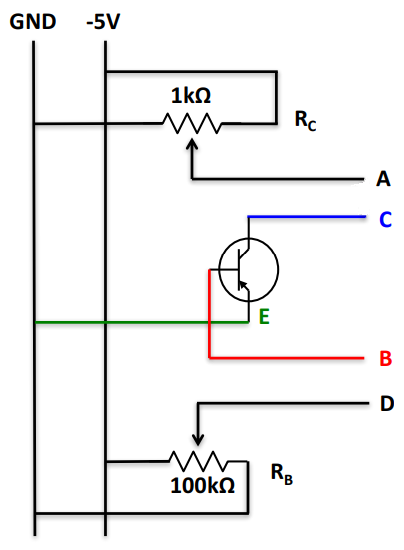
\includegraphics[width=0.5\linewidth]{pictures/circuito.png}
    \caption{Caption}
    \label{fig:circuito}
\end{figure}

\begin{figure}
    \centering
 %   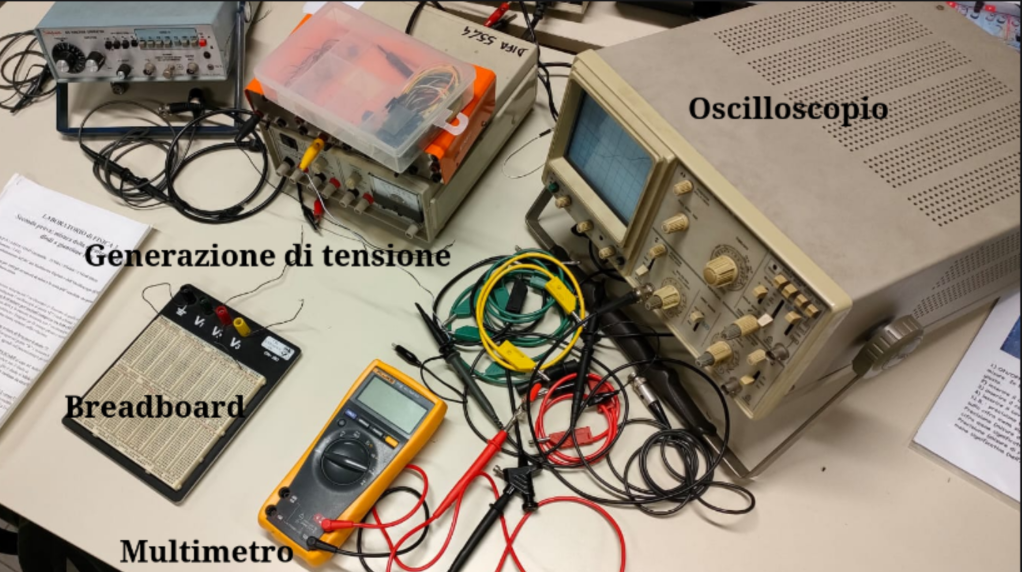
\includegraphics[width=0.5\linewidth]{pictures/apparato.png}
    \caption{Caption1}
    \label{fig:apparato}
\end{figure}


\section{Risultati}



\subsection{Dati}


\begin{table}[h!]
\centering
\begin{tabular}{|c|c|c|}
\hline
\textbf{par 1} & \textbf{par 2} & \textbf{par 3} \\
\hline
a & b & c \\
\hline
d & e & f \\
\hline
g & h & i \\
\hline
\end{tabular}
\caption{Ho imparato l'alfabeto ma nemmeno tutto}
\label{}
\end{table}


\subsection{Analisi Dati} 
Nella figura si mostra il risultato dell'onda di potenziale tosata nel caso di confurazione con diodi al silicio

\begin{figure}
	\centering
	%   \includegraphics[width=0.5\linewidth]{pictures/onda_tosata.png}
	\caption{Caption1}
	\label{fig:apparato}
\end{figure}



\section{Conclusioni}



\medskip

\printbibliography

\end{document}